%# -*- coding: utf-8-unix -*-
%%==================================================
%% intro.tex for SJTU Master Thesis
%%==================================================

%\bibliographystyle{sjtu2}%[此处用于每章都生产参考文献]
\chapter{绪论}
\label{chap:intro}

本章是课题的绪论部分。在本章节中,首先介绍了课题的实际背景,之后总结了课题的研究目的与研究意义,并对国内外对于本次课题相关的研究现状进行了分析。最后介绍了本次课题研究的主要内容。

\section{课题背景}

目前,容器虚拟化的风潮正在席卷全球。容器虚拟化,又被称作操作系统级别的虚拟化。是指操作系统的内核允许多个相互隔离的用户态进程同时执行,这些用户进程会被称为容器,它们共享一个操作系统内核。这样的技术在2000年左右就出现了,比如FreeBSD jail,Virtuozzo等等都是操作系统级别的虚拟化工具。但是容器虚拟化最近才渐渐地变得广为人知,是因为Docker在2013年的发布。Docker是由PAAS服务商DotCloud实现的开源容器工具,其很好地解决了容器的构建,落地和运行的全流程,采用了很多对开发友好的技术使得容器虚拟化变得更加易用。

因为容器虚拟化技术重新进入业界的视野,整个世界的软件企业,都或多或少受到了容器技术的影响。在容器的影响下,很多经典的软件工程的概念都有了新的内涵与实现。在软件开发过程中,版本的管理与发布是一个非常值得讨论的话题。其中版本管理是指对于文件的修改可以被记录,而且可以在合适的时候进行回滚的技术,是对于文件的修改记录进行管理与控制的过程。而软件的版本发布,可以被理解为当软件的全部或者部分特性可以被交付时,进行的对软件进行发包并发布的过程。在目前的软件开发流程中,软件的过程往往是迭代的。项目组的成员会针对具体的需求规约,将软件需要实现的功能划分,迭代地去完成,而不再是如同传统的瀑布流开发过程,在软件功能全部实现后才会发布一个新版本。这样的变化就对版本管理与发布有了新的要求,要求版本的管理与发布要是持续的过程。于是持续集成与持续部署的概念就应运而生。

持续集成,是一种软件工程中的实践,是指持续性地将所有开发者的代码合并到一个主要的分支中的过程。其目的是为了防止软件中因为代码集成而可能造成的问题。其概念最早是由Grady Booch在1991年提出。\cite{Booch}后来持续集成作为一种实践被引入XP敏捷过程中,目前持续集成已经越来越被业界认为是软件工程中保证代码质量与交付可靠性的一种必要实践。持续集成带来的好处是显而易见的,它使得软件测试时间提前了,融入到了每次代码的改动中。同时为持续部署提供了可能性,同时也降低代码复查的时间。因此很多版本控制与发布的网站,诸如Github,Gitlab等都提供了对持续集成的支持。持续集成的概念也不再仅限于敏捷过程中。

而持续部署,是一个为了解决软件发布引起的问题而提出的概念。持续部署是持续集成的一种扩展,指持续性地将代码部署到生产环境中的过程。在传统的软件过程中,软件的发布是非常繁杂而且易错的事情。因为在发布的过程中,涉及到对代码的打包,运行时环境的依赖以及配置管理等等。所以在传统的发布过程中,是耗时耗力的。而持续部署,就是希望能够降低发布新版本带来的额外成本,使得发布不再是一个高成本的过程。\cite{CruiseControls}

因为持续集成与持续部署,都涉及到环境的隔离等,因此在容器虚拟化技术出现之前,持续集成与持续部署往往是采用虚拟机,或自定义的隔离手段来实现每次集成与部署之间的资源隔离。而在容器虚拟化技术走向成熟后,持续集成与持续部署也有了新的一种实现手段。

容器虚拟化技术,不仅对于持续集成与持续部署的内涵有了新的定义,也因此应运而生了基于容器的机器集群。在真实的环境中,单个服务器往往是不能保证服务的可用性的,所以往往会引入多台服务器,而这就会涉及到集群管理的技术。通过使用集群的方式,引入更多的冗余资源来保证服务的可用性,是目前比较常用的手段。而在容器虚拟化技术出现之前,业界通常会采用Mesos或者其他的集群管理工具,来调度集群上的任务,来保证在尽量不浪费集群的计算能力的同时做到高可用。而这样的集群管理工具管理的单元往往是虚拟机,相较于容器而言,虽然有着更好的隔离性,但却不如容器灵活。而随着谷歌关于其容器集群管理工具的论文发表\cite{Borg},原本的集群管理工具也开始拥抱容器。容器所具有的灵活,轻量的特点,使得它天然契合生产环境中的某些应用场景。

\section{Docker容器技术}

Docker是一个开源的容器虚拟化工具,它可以帮助开发者便捷地进行容器的构建,发布,与运行。本部分将从容器技术本身,Docker的核心概念,以及Docker的架构,相比于其他容器的工具而言的优势四个部分来介绍Docker这一容器虚拟化工具。

\subsection{容器虚拟化技术概览}

\begin{figure}[!htp]
  \centering
  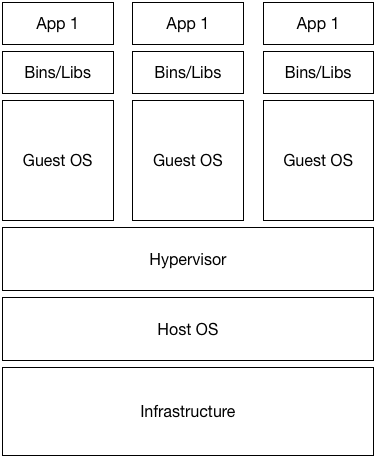
\includegraphics[width=0.4\textwidth]{tech/vm.png}
  \bicaption[fig:vm]{传统虚拟化技术示意图}{传统虚拟化技术示意图}{Fig}{}
\end{figure}

容器虚拟化技术并不是一个最近才出现的新技术,而是在2000年左右就已经有不少应用的虚拟化手段。

在容器虚拟化技术之前,比较常用的虚拟化工具有Xen,VMware等等。这些虚拟化工具都是属于Application Binary Interface级别的虚拟化,这样的虚拟化技术允许多个操作系统同时运行在同一套硬件上。这样的实现方式往往需要一个Virtual Machine Monitor,或者称作VMM的系统,来将硬件资源进行虚拟化,将虚拟机运行在虚拟化后的设备上。

而容器虚拟化技术是属于Application Programming Interface级别的虚拟化,每一个虚拟机,也被称为容器,只是操作系统上的一个进程,与普通的进程不同,容器使用namespace等等方式来将资源隔离,使得进程之间互相不感知。\cite{soltesz2007container}

相比于传统的虚拟化方式,容器虚拟化更加轻量,启动和销毁的速度快,资源消耗少。但与此同时,容器虚拟化也存在一些问题,首先是使用容器虚拟化的技术虚拟出来的容器,共用操作系统的内核。因此如果容器内导致了内核崩溃,那会影响到其他的容器。而使用Xen等技术,一个虚拟机的崩溃对于其他虚拟机而言,不会有任何影响。\cite{dua2014virtualization}

\subsection{Docker的核心概念}

Docker是目前被广泛接受的一种容器虚拟化工具,其有着其他容器虚拟化工具所不具备的一些优势。Docker原本是DotCloud公司的一个内部项目,DotCloud是一个专注于平台即服务的创业公司。在2013年3月13日,Docker发布了它的开源版本。它使用了内核中的lxc作为其容器的支持,同时还使用了内核中的cgroups和namespace的特性,因此需要内核支持。在Docker开源后,因为其便捷和高效的特性,受到了开发者的欢迎。在最初的版本中,Docker的网络等方面还不是特别的完善,但是Docker由DotCloud公司进行积极的开发和维护,在2014年的0.9版本中,Docker移除了lxc的依赖,直接与内核中的特性进行交互。并且亚马逊、IBM、微软Azure等等国际云服务提供商纷纷表示将整合Docker技术到其云计算产品中,一时之间Docker成为了云计算领域的热词。截止至2016年5月16日,Docker在Github上收获了31256个关注(Star),成为了Github上最受欢迎的项目之一。

\begin{figure}[!htp]
  \centering
  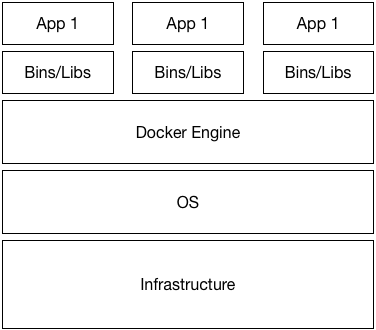
\includegraphics[width=0.4\textwidth]{tech/container.png}
  \bicaption[fig:container]{Docker示意图}{Docker示意图}{Fig}{}
\end{figure}

如图\ref{fig:container}所示,Docker不同于传统的虚拟化技术,每一个容器包含其运行时需要的所有依赖以及应用,但并不需要一个虚拟机来提供支持,每一个Docker容器只是一个运行在独立的namespace下的受到隔离的进程。与此同时,Docker容器不会跟下层的操作系统相耦合,它们可以运行在所有支持Docker Engine的机器或者云上。

Docker中比较重要的两个概念分别是镜像和容器,这是Docker最主要的两个实体概念。镜像是Docker的一个特色,镜像是一个只读的模板,在启动容器时被加载。镜像在存储方面,采取了联合文件系统。联合文件系统允许系统的文件和目录以分层的方式存储,而对于操作系统而言,其使用的文件系统是分层叠加之后的结果。这样使得镜像的存储变得更加方便,可以将不同的文件分层并行地进行上传或下载。而且当对镜像进行修改时,只需要对修改之后的文件分层进行添加或者修改即可,而不需要替换掉整个镜像。而Docker通过定义了一系列操作,将镜像的构建进行了标准化,使得用户只需要通过简单地操作,即可构建出满足自己需要的镜像。\cite{mayue}

而容器则是镜像的运行时,镜像为容器提供了启动的环境,而容器则与常规的容器虚拟化技术中的容器概念一致,是一个隔离的进程。因为Docker的镜像是一个只读的模板,其所有的文件分层都是设置为只读的,因此当从一个镜像运行起一个容器时,Docker会在镜像的最上层添加一个可读可写的新的文件分层。在新的文件分层中对于文件系统的修改,会覆盖原本的镜像。这样就使得容器看起来运行在镜像之上,而并不会因为容器的运行修改镜像的内容。

\subsection{Docker的架构}

\begin{figure}[!htp]
  \centering
  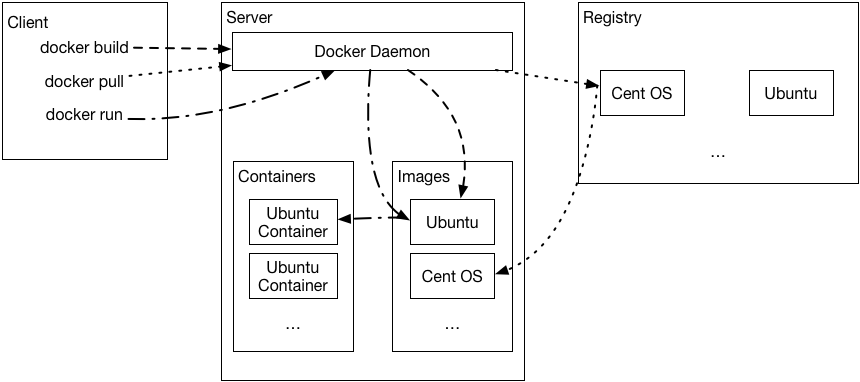
\includegraphics[width=\textwidth]{tech/architecture.png}
  \bicaption[fig:architecture]{Docker架构图}{Docker架构图}{Fig}{}
\end{figure}

如图\ref{fig:architecture}所示,Docker采取了客户端-服务器的架构。其中比较重要的组件有Docker Daemon,Docker Client,Docker Registry三个,下面将从镜像和容器的生命周期角度,对Docker的架构进行介绍。

Docker Daemon,是运行在服务器端的后台程序。其承担了基本所有的操作,包括本地镜像和容器的管理,与远端的Docker Registry的交互等等。但用户并不直接与Docker Daemon交互,而是通过Docker Client。Docker Client是一个Cli程序,为用户提供了抽象度很高的命令,通过Docker Client,用户可以与Docker的服务器进行交互,进而管理容器和镜像。而Docker Registry是管理镜像的存储组件,用户可以将构建好的镜像推送至Docker Registry中,而通过Docker Client,用户可以对Docker Registry上的镜像进行简单的搜索,寻找适合自己应用场景的镜像,并拉取使用。

Docker有一系列优秀的特性。首先,作为一个容器虚拟化工具,它允许用户创建Docker容器,并且利用iptable等等特性,解决了容器与容器之间互相连接的问题。同时,Docker允许构建镜像,并且可以将镜像推送给远端的Registry,这使得一次构建,多次运行的想法成为了现实。而且Docker的Registry允许多租户,通过类似Github的方式来进行组织与构建,使得Docker在生产环境的使用成为了可能。

除此之外,Docker的成功也离不开其强大的生态环境。围绕着Docker,有一系列工具和技术覆盖了当下很多领域的难题。首先,Docker周边有非常多为了降低Docker的使用门槛的工具,比如Docker Machine等。原本因为容器虚拟化技术需要依赖Linux内核的某些特性,使得其他系统的用户不能使用Docker来构建容器,但是Docker Machine会在非Linux环境下运行一个Linux虚拟机,将Docker运行在该虚拟机上,这抹平了Docker对内核的要求,使得其他系统的用户也可以自如地使用Docker来构建容器,目前Docker正在积极基于OS X的新特性积极地进行对OS X系统的原生支持,这对于OS X系统的用户而言是一大利好。其次,Docker跨平台的特性,使得企业的混合云部署变成了现实。面对当下异构的机器和网络环境,Docker能够更好地发挥其特性。除此之外,在持续集成与持续部署方面,Docker非常用来做环境的隔离,执行构建任务。Drone等工具就是专注于该领域的,基于Docker来实现的工具。

\section{国内外课题相关研究现状}

在容器虚拟化技术出现后,基于容器的持续集成工具也随之产生。Drone是一个在Github上开源的,使用golang实现的基于Docker的持续集成工具,它的目标是取代Jenkins成为新一代的持续集成工具。相比于Jenkins,Drone本身更加简洁,而且同样有丰富的插件支持。Drone更加倾向简洁,专一的设计,Drone的实现中没有调度的概念,而鼓励用户通过cron等工具的方式来实现定时触发构建任务等功能。而且Drone使用Docker容器来进行构建并执行用户定义的脚本,将进行资源隔离的方式和手段与持续集成工具本身解耦,相比Jenkins而言有着更先进的实现以及更加活跃的社区。目前Drone在Github上已经收获了六千多个关注,其受欢迎程度由此可见一斑。

而对于持续部署而言,业界采取的方式相对统一,是将继续部署与持续集成结合在一起去完成的。在持续集成完成后,如果确认代码变动没有问题,就将代码自动化地部署到服务器上。以Drone为例,它对于部署的实现方式是允许用户在持续集成后,根据集成测试的结果来决定是否将新的变动发布到生产服务器上。

\section{研究的目的与内容}

本文希望能够结合容器虚拟化技术与版本管理与控制的技术,实现一个基于容器虚拟化技术和容器集群技术的版本管理与发布系统Fornax(以下统一称为Fornax),使得用户能够在容器集群上进行代码的版本管理与发布。

Fornax的目的在于方便使用容器集群的开发者的开发过程,使得开发者在不感知底层容器集群的行为的情况下,完成应用的持续集成与持续部署。在遇到问题需要回滚或者升级时,也可以通过Fornax来进行相应操作。开发者只需要关注业务逻辑的开发,由Fornax完成部分冗杂的运维操作。

Fornax希望能够实现三个主要特性:对于代码的持续集成,对于应用的持续部署持续发布,以及对于用户应用的版本管理。

在容器虚拟化技术出现之前,对于应用的版本管理只需要使用git等工具,保证对于代码的每次修改都被记录下来并且可回滚即可,而在容器虚拟化技术出现之后,对于一个容器化的应用而言,不仅需要对代码进行版本管理,也需要对容器的镜像进行管理。Fornax希望能够将每次可运行的代码,打包为一个容器镜像,并且对镜像如同代码一样进行版本管理。这样不仅可以保证在发布出现问题时,更好地对代码和运行环境进行回滚,而且也可以使得发布环境可追溯。

在持续集成方面,Fornax希望支持根据每次代码的变动来自动地发起一次集成。每当代码发生了变动时,Fornax会检查配置文件中关于持续集成的配置与设定,来根据用户自定义的脚本来发起一次集成,并将集成的日志和结果持久化地记录下来。在持续集成时,会使用容器技术来保证集成时的环境隔离。同时,对于在运行时的依赖,Fornax也希望通过容器的方式来给予支持。\cite{wangfei, zhangjian}

在持续部署方面,Fornax希望可以基于Kubernetes容器集群进行实现。Kubernetes是一个基于Docker的容器管理工具,由谷歌开源,因为谷歌在2015年发布的论文\cite{Borg}而被人所知。不同于其他的集群管理工具,它将一个或多个容器的组合作为基本的调度单位。Fornax希望基于Kubernetes进行对于用户的应用的持续部署与持续发布。每当用户代码的集成测试结束后,会根据持续集成的结果来进行相应的代码部署,用户可以在配置文件中关于持续部署的设定中写明代码部署对应的集群等。

Fornax主要的功能是以上三点,而除此之外,还有一些非功能的要求。首先,因为Fornax面临的环境可能是异构的,可能会部署在公有云、私有云或者是混合云上,因此Fornax需要是可配置的,而且应该支持跨平台。在不同的环境上都可以为用户提供服务。除此之外,因为不同的用户对于持续集成和持续部署的要求与使用方法都是不同的,因此,在Fornax的实现上,要允许用户自定义在持续集成等环节的行为。

\section{论文结构}

本文一共由五章组成。

其中第一章为绪论部分,主要介绍了本文的研究背景,有关持续集成、持续部署在工业界的情况,容器虚拟化技术的相关研究分析以及本文的研究目的与内容。

第二章对Fornax进行了总览性的介绍。首先从需求方面对Fornax进行了分析,明确了Fornax要实现的功能,接下来对Fornax的实现架构进行了阐述,并说明确定以这样的架构实现的原因。

第三章详细阐述了Fornax的具体实现。其中详细介绍了对于实现难度比较大的两个模块:持续集成模块与日志模块。并在对各个模块的实现分析中,分析了采取这样的实现方式的原因。

第四章是验证与测试部分。在该部分中介绍了Fornax的测试架构与分布式部署的探索。

第五章是总结部分,在该部分中总结了本文做的主要工作,以及在之后Fornax需要继续完善的问题。